\definecolor{myblue}{RGB}{80,80,160}
\definecolor{mygreen}{RGB}{80,160,80}
\usetikzlibrary{positioning,chains,fit,shapes,calc}

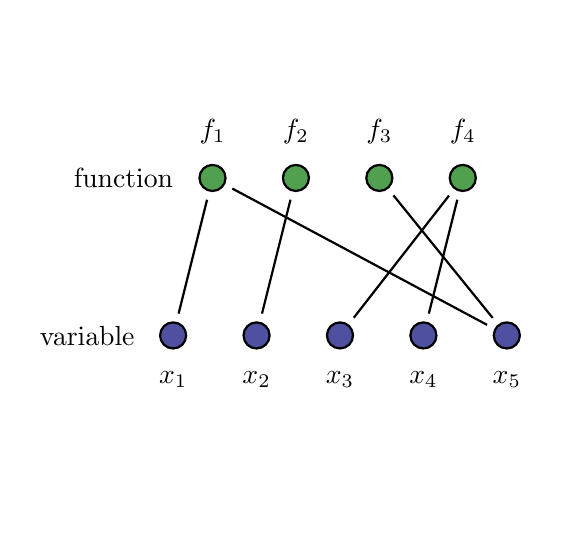
\begin{tikzpicture}[thick,
  every node/.style={draw,circle},
  fsnode/.style={fill=myblue},
  ssnode/.style={fill=mygreen},
  every fit/.style={draw=none},
  shorten >= 3pt,shorten <= 3pt
]

% Function
\begin{scope}[start chain=going right,node distance=7mm]
\foreach \i in {1,2,...,5}
  \node[fsnode,on chain] (x\i) [label=below: $x_\i$] {};
\end{scope}
\node [myblue,fit=(x1) (x5),label=left:variable] {};

% Coordinates
\begin{scope}[yshift=2cm,xshift=.5cm,start chain=going right,node distance=7mm]
\foreach \i in {1,2,...,4}
  \node[ssnode,on chain] (f\i) [label=above: $f_\i$] {};
\end{scope}
\node [mygreen,fit=(f1) (f4),label=left:function] {};

% Edges
\draw (x1) -- (f1);
\draw (x2) -- (f2);
\draw (x3) -- (f4);
\draw (x4) -- (f4);
\draw (x5) -- (f1);
\draw (x5) -- (f3);
\end{tikzpicture}